\newpage
\section{Factorial Hidden Markov Models}

この章ではFactorial Hidden Markov Modelsについて説明する.
EMアルゴリズムや変分推論\cite{variational_method}などを用いたパラメータ推定など,更に詳細な内容については参考文献\cite{fhmm}を参照されたい.

\subsection{モデル概要}
Factorial Hidden Markokv Models(FHMM)\cite{fhmm}は1997年に提案された,
複数の隠れ変数のマルコフ連鎖に対応したHMMであり,
音声解析や自然言語処理,モーションキャプチャによる運動データの復元など提案されてから今日まで多岐にわたり利用されている\cite{s_f_fhmm, Logan97factorialhidden, Dongheui2008missing, NepalY13}.
FHMMでは,互いに独立な複数の隠れ変数のマルコフ連鎖があり,ある時刻$t$における観測変数は,時刻$t$におけるすべての隠れ変数の状態に依存する.
図\ref{fig:fhmm}に対応するグラフィカルモデルを示す.このグラフィカルモデルでは,時刻$t$における$m$個目のマルコフ連鎖の隠れ変数を$S^{(m)}_{t}$,
観測変数を$x_{t}$としている.

\begin{figure}[t]
  \centering 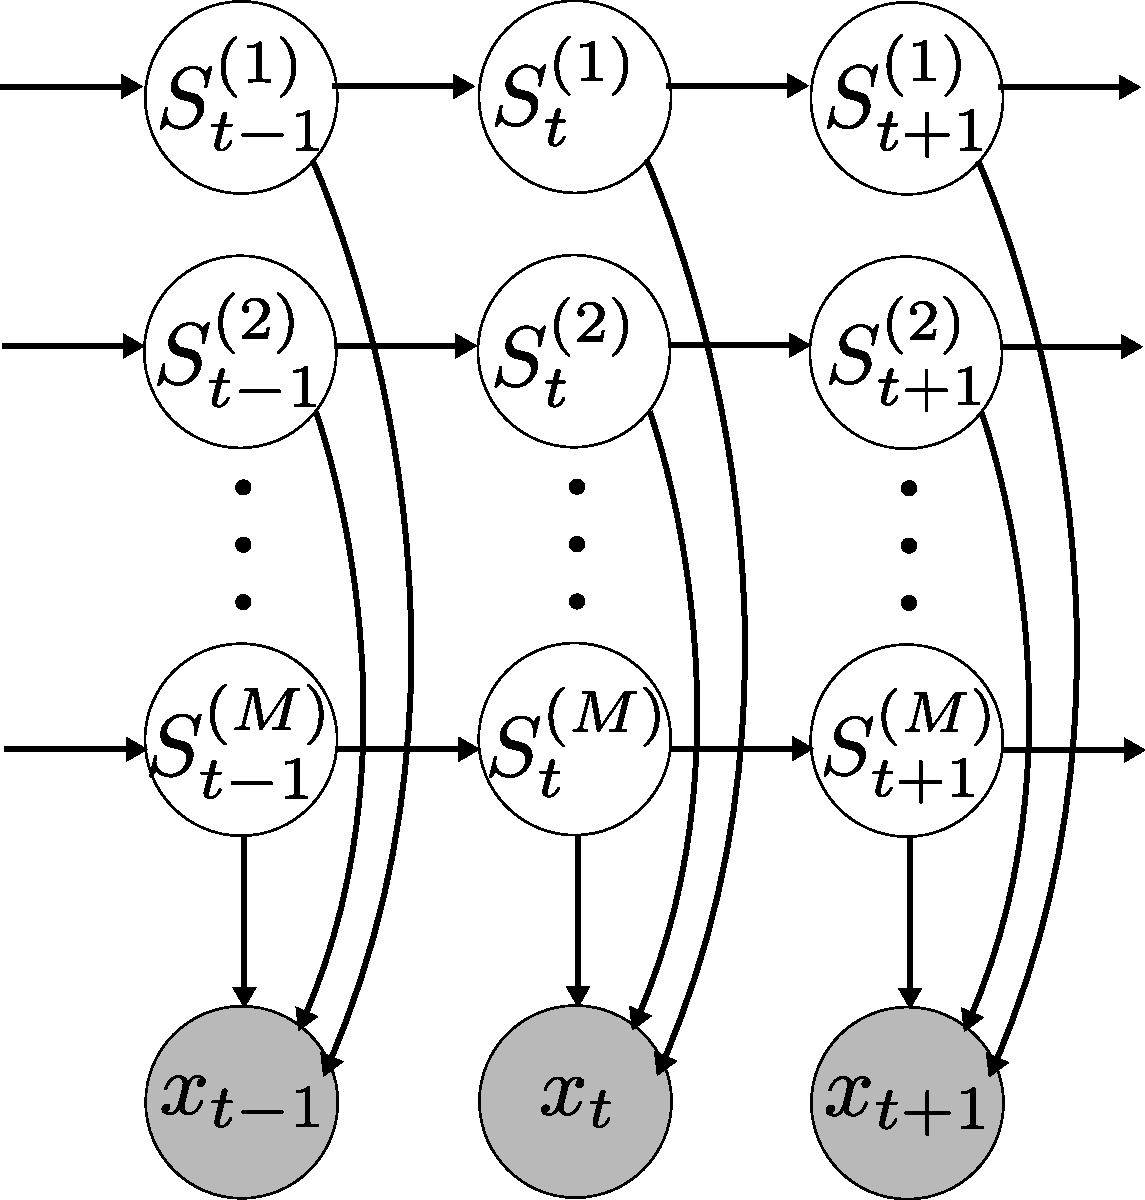
\includegraphics[width=0.5\hsize, bb=0 0 550 576]{fhmm.pdf}
  \caption{FHMMのグラフィカルモデル}
  \label{fig:fhmm}
\end{figure}

\subsection{確率モデル}
まず,通常のHMMの場合を考える.
状態系列
\begin{equation}
  \mathbf{s} = s_{1}s_{2}\cdots s_{t} \cdots s_{T}
\end{equation}
と観測系列
\begin{equation}
  \mathbf{x} = x_{1}x_{2}\cdots x_{t} \cdots x_{T}
\end{equation}
を考える.
このとき,式(\ref{eq:p_x_s})は,
\begin{equation}
  P(\mathbf{x}, \mathbf{s}) = P(s_{1}) P(x_{1} | s_{1}) \prod_{t=2}^{T} P(s_{t} | s_{t-1}) P(x_{t} | s_{t})
\end{equation}
と書ける.ただし,状態数を$K$としたとき,
\begin{equation}
  s_{t} \in \{1, ..., K\}
\end{equation}
である.このとき,HMMの遷移確率行列$P(s_{t} | s_{t-1})$は$K \times K$になる.
また,出力記号の数を$D$としたとき,HMMの出力確率行列$P(x_{t} | s_{t})$は$K \times D$になる.
出力確率行列$P(x_{t} | s_{t})$が連続値をとる場合,正規分布(ガウス分布)や混合正規分布,またはニューラルネットワークのような多くの異なる形でモデル化することができる.


次に,FHMMの場合を考える.FHMMでは複数の隠れ変数のマルコフ連鎖があるので,時点$t$における隠れ変数は,
\begin{equation}
  s_{t} = s_{t}^{(1)},s_{t}^{(2)},\cdots, s_{t}^{(m)}, \cdots, s_{t}^{(M)}
\end{equation}
と表せる.ここで,隠れ変数のマルコフ連鎖の数を$M$とした.
各状態変数$s_{t}^{(m)}$は,$K^{(M)}$個の状態をとる.しかし本誌では簡略化のため,すべての$m$に対して$K^{(M)} = K$とする.
このとき,遷移確率行列$P(_{t} | s_{t-1})$を次のように表す.
\begin{equation}
  P(s_{t} | s_{t-1}) = \prod_{m=1}^{M} P(s_{t}^{(m)} | s_{t-1}^{(m)})
\end{equation}

図\ref{fig:fhmm}を見ると,時点$t$における観測値$x_{t}$は時点$t$におけるすべての隠れ変数に依存していることがわかる.
連続値をとる観測値のために,これらの依存を解決する手法の1つとして線形ガウスモデル(Liner Gaussian Model)がある.
これは,観測値$x_{t}$が正規乱数ベクトルになっており,その平均が状態変数の線形関数になっているものである.
ここで,状態変数を1-of-K表現で表すこととする.1-of-K表現とは,K番目の要素が1でそれ以外の要素はすべて0であるベクトル表現である.

$D \times 1$の観測値ベクトルの確率分布は,
\begin{equation}
  P(x_{t} | s_{t}) = |C|^{-\frac{1}{2}} (2\pi)^{-\frac{D}{2}} \exp \left\{- \frac{1}{2} (x_{t} - \mu_{t})^{\top} C^{-1} (x_{t} - \mu_{t}) \right\}
\end{equation}
で表される.ここで,
\begin{equation}
  \mu_{t} = \sum_{m=1}^{M} W^{(m)} s_{t}^{(m)}
\end{equation}
とする.
各行列$W^{(m)}$は$D \times K$の行列であり,その列は各$s_{t}^{(m)}$を決める平均に寄与するものであり,
$C$は$D \times D$の分散・共分散行列,$^{\top}$は転置,そして$| \cdot |$は行列式を表す.
